% !TEX encoding = UTF-8 Unicode
% discussion

In this thesis project, the tissue-specific function of PPP2R5C has been shown at the first time by the hepatocyte-specific knockdown of PPP2R5C both \textit{in vitro} and \textit{in vivo}. From the Expression Altas database at EBI, although the liver is not the organ having the highest PPP2R5C expression comparing to the heart, brain, testis and thymus, \textit{in vivo} liver knockdown of PPP2R5C changes the mouse metabolism profoundly. The profound change in metabolism, from the glucose uptake to lipogenesis, is likely resulting from multiple actions of PPP2R5C on its substrates. And the substrate multiplicity in metabolism control makes PPP2R5C a novel and interesting drug target in developing pharmaceuticals for controlling hyperglycemia and hyperinsulinemia in the future. Further characterization of the gene regulation in PPP2R5C is also an interesting topic open for new mechanism in etiology of diabetes, especially with the fact that the PPP2R5C is misregulated in the type 2 diabetes and has predicted HNF1\textalpha{} and \gls{nfkb} sites on its promoter. Both HNF1\textalpha{} and chronic inflammation has been linked to the development of diabetes \cite{owen_monogenic_2013,patel_role_2009}.   

\section{PPP2R5C in liver metabolism}

PPP2R5C, a PP2A regulatory subunit, is identified as a metabolism modulator in hepatocytes. Reduced PPP2R5C expression leads to the increased glucose uptake, glycolysis and \textit{de novo} lipogenesis in \textit{in vitro} cultivated hepatocytes and mouse hepatoma cell line. These phenotypes are recapitulated \textit{in vivo} whereby liver-specific knockdown of PPP2R5C in mice results in the  improved glucose tolerance and insulin sensitivity, but elevated circulating \gls{vldl} levels (Figure~\ref{fig:fig2.56}). The phenotypes presented in this thesis were obtained by knocking down PPP2R5C with multiple independent miRNA or shRNA sequences (See Table~\ref{tab:tab7}) and different shRNA/miRNA expression systems, including \gls{AV}, \gls{AAV} and piggyBac inducible system. For instance, the increased glucose uptake was observed in cell culture using two independent shRNAs (Figure~\ref{fig:fig2.14}) and a third independent target sequence \textit{in vivo} (Figure~\ref{fig:fig2.43}). This excludes the possibility that the phenotypes could arise from possible off-target effects or virus-mediated effects. 


Therefore, PPP2R5C is a fine-tuning regulator for adjusting the balance liver has to make, which is the equilibrium between preventing circulating glucose levels from becoming too elevated in the postprandial phase (alternatively, high oral or enteral glucose load, such as that in GTT), and yet not flooding the circulatory system with lipids. With higher expression of PPP2R5C in the liver, mice would end with less glucose uptake and eventually less lipid secretion to the circulation. However, the glucose uptake in other tissues, such as muscle and adipose tissues, need cooperatively increase their glucose absorption in order to control the mild hyperglycemia in the postprandial phase or other conditions with massive glucose load. With less expression of PPP2R5C in the liver, liver will relieve the glucose uptake burden for other tissues, such as muscle and adipose tissues, but will release more lipid into circulation and have long-term risk for cardiovascular diseases in the expense of better insulin sensitivity and improved glucose tolerance. These scenarios could make fine-tune of the PPP2R5C expression level a tough choice for mouse liver during evolution. Mice have to evolve an appropriate level of PPP2R5C expression to have a balanced glucose uptake and lipid secretion in the liver.

Interestingly, PPP2R5C liver-specific knockdown mice have reduced levels of serum insulin (Figure~\ref{fig:fig2.28}) but normal levels of circulating glucose (Figure~\ref{fig:fig2.26}) under various feeding conditions. One possible reason for the reduced insulin level can be that the pancreas, which is the central control unit for the euglycemia in the body, is not affected in PPP2R5C liver-specific KD mice. Consequently, the pancreas is still remaining its blood glucose controlling function normally to maintain a proper blood glucose level, reducing its insulin secretion to compensate for the elevated glucose clearance by the liver. 

Due to the increased VLDL secretion in fasting and refed conditions, steady-state triglyceride level in the liver shows a decrease in fasting and no further increase in refed, unlike the increased triglyceride during \textit{ad libitum} feeding. Given the continuous consumption of triglyceride from circulating VLDL by adipose tissues, muscle and other peripheral tissues during fasting, the overall triglyceride production in the liver could still be increased. This hypothesis could be further resolved by \textit{in vivo} tracer study to clarify how much isotope-labelled glucose is converted into the liver and serum triglyceride. During refed, the combined triglyceride from liver and serum are increased upon PPP2R5C KD, and the liver triglyceride was increasing faster than control during re-accumulating triglyceride after fasting (Figure~\ref{fig:fig2.56}). The evidence demonstrated the general function of PPP2R5C in inhibiting lipogenesis during all feeding regimes (at least for \textit{ad libitum} feeding and refed). Another consequence after the increased VLDL secretion is that liver cholesterol levels drop significantly during fasting and refed (Figure~\ref{fig:fig2.35}). The decreased level of cholesterol could also contribute the SREBP-1 activation in the liver (\cref{fig:fig2.52,fig:fig2.55}), since cholesterol is an endogenous inhibitor for SREBP-1 activation \cite{wang_srebp-1_1994}. 


\begin{figure}[!tb]
\centering
\includegraphics[width=0.8\textwidth]{figs/fig2-56 whole organismal model.png}
\caption[Whole organismal model for PPP2R5C's metabolic control]{\footnotesize Whole organismal control model for PPP2R5C in glucose and lipid homeostasis in liver. Upon PPP2R5C knockdown in liver, glucose uptake is increased in the postprandial phase or high glucose load during GTT. Glucose in the liver is quickly converted to glucose-6-phosphate in order to stay in the liver. The absorbed glucose is further stored either as glycogen or triglyceride. Increased triglyceride storage triggers VLDL secretion and results in passively lowering liver cholesterol. During fasting, the higher rate of VLDL secretion could cause the decreased liver triglyceride, while increased triglyceride synthesis rate during refeeding balances triglyceride production and secretion from liver and results in no net change in liver steady-state triglyceride level.}
\label{fig:fig2.56}
\end{figure}

In short term, reducing PPP2R5C levels in liver seems to have a beneficial role in whole organismal level (Figure~\ref{fig:fig2.56}). The liver becomes more capable of glucose deposition in the postprandial phase, and reducing the relative glucose burden on other insulin-sensitive glucose uptake tissues such as adipose tissues and muscle. This feature could be employed in controlling hyperglycemia in metabolic syndromes. The long-term reduction in liver PPP2R5C, which has been shown in knockout mice for PPP2R5C \cite{varadkar_protein_2014}, results in the obesity in mice. Although the reason for the obesity in whole body knockout mice can not be solely attributed to the liver, the increased VLDL secretion from liver-specific knockdown mice raises the risk of developing obesity and cardiovascular diseases. However, the long term consequence of PPP2R5C manipulation still need to be carefully investigated. 


\section{PPP2R5C substrates}

Although the phenotypes after PPP2R5C knockdown, the increased glycolysis and lipogenesis, are quite specific both in cell culture and \textit{in vivo} mouse experiment. However, they are still could be a result from the effects of PPP2R5C on multiple downstream substrates. Thus, it will be difficult or even impossible to pin down single one PPP2R5C's substrate as the main mechanism for explaining most of the effects of PPP2R5C KD. Here 4 protein complexes were identified as PPP2R5C interacting partners including AMPK, HIF1\textalpha{}, STAT3 and S6K. I tested whether the phosphorylation of these proteins increases upon PPP2R5C knockdown, which would be the expected result from a PPP2R5C target. 

For STAT3, I used the phospho-specific antibody for S727 of STAT3 to check the phosphorylation change upon PPP2R5C KD, and there was no change in two independent inducible shRNA mediated KD (data not shown). Again, I used the Phos-tag\textsuperscript{\textregistered} gel  to test STAT3's motility shift due to increased phosphorylation in an approach similar to what I did for HIF1\textalpha{} (Figure~\ref{fig:fig2.51}). Although there were no obvious changes in STAT3's motility, an important caveat of Phos-tag\textsuperscript{\textregistered} from my experience is that Phos-tag\textsuperscript{\textregistered} gels could only resolve phosphorylations on roughly one third of the proteins I have tested and know to be phosphorylated. There is still possibility that STAT3 is differentially phosphorylated after PPP2R5C KD.

For S6K, I also checked the phosphorylation of Thr389 by using commercially available phospho-specific antibody. It was not up-regulated upon PPP2R5C knockdown. Also, I evaluated the S6K phosphorylation on other sites  by Phos-tag\textsuperscript{\textregistered} gel, and the result was hard to explain the existence of band shifting due to multiple bands for S6K. The multiple bands separated on Phos-tag\textsuperscript{\textregistered} gel would potentially mask some changes. For this reason, S6K branch was not explored in depth, although this does not exclude the possibility of PPP2R5C's regulation on S6K's other site phosphorylation. For these reasons, I focused more on AMPK and HIF1\textalpha{} for deciphering PPP2R5C's role in metabolism control.

For AMPK and HIF1\textalpha{}, I evaluated both the phosphorylation and activity of them upon PPP2R5C knockdown. Both AMPK and HIF1\textalpha{} are known to increase the glycolytic flux in response to stress conditions, either imbalanced ATP/ADP ratio or impaired mitochondrial function \cite{hardie_ampk:_2012,denko_hypoxia_2008}. Therefore AMPK and HIF1\textalpha{} tend to work in concert to promote the glucose uptake and glycolysis upon PPP2R5C knockdown (Figure~\ref{fig:fig2.59}). For PPP2R5C's control in the glucose uptake and glycolysis branch, at least in Hepa 1-6 cells and primary hepatocytes, AMPK activity and its downstream effector in glucose uptake--TBC1D1 phosphorylation are shown to be increased. TBC1D1 phosphorylation is known to be a critical mediator in glucose uptake stimulation followed from AMPK activation, and its phosphorylation at Ser700 and Ser660 sites are \textit{bona fide} AMPK target \cite{vichaiwong_contraction_2010}. Both glut1 and glut4 translocation have been shown to be regulated by TBC1D1 phosphorylation. However, glut2 is the highest expressed glucose transporter in hepatocytes, while glut1 or glut4 is lowly expressed, and glut1 is only expressed in sinusoidal membrane of hepatocytes with its protein restricted to hepatocytes proximal to the hepatic port venule \cite{karim_hepatic_2012}. The expression pattern of glut1 in the liver indicates TBC1D1 mediated glut1 translocation could potentially play a role in glucose uptake at port vein where massive glucose load is encountered in the postprandial phase or enteral glucose overload. 

Indeed, the \textit{in vivo} function of AMPK has also been carefully investigated in the mouse liver, which is the increased liver AMPK activity leading to the decreased blood glucose and fatty liver \cite{foretz_short-term_2005}. The reduced liver AMPK activity leading to a glucose intolerance \cite{andreelli_liver_2006}, in agreement with the potentially increased AMPK activity upon PPP2R5C KD. However, the activation of AMPK phosphorylation at Thr172 has not been observed in the mouse liver sample after PPP2R5C KD. Only ACC1 phosphorylation increase has been observed, yet with increased total ACC1 (data not shown). Although the phenotype of increased glucose uptake \textit{in vivo} is still fit with potentially activated AMPK, it is inevitable that other mechanisms downstream of PPP2R5C are also contributing to glucose uptake phenotype.

\begin{figure}[!tb]
\centering
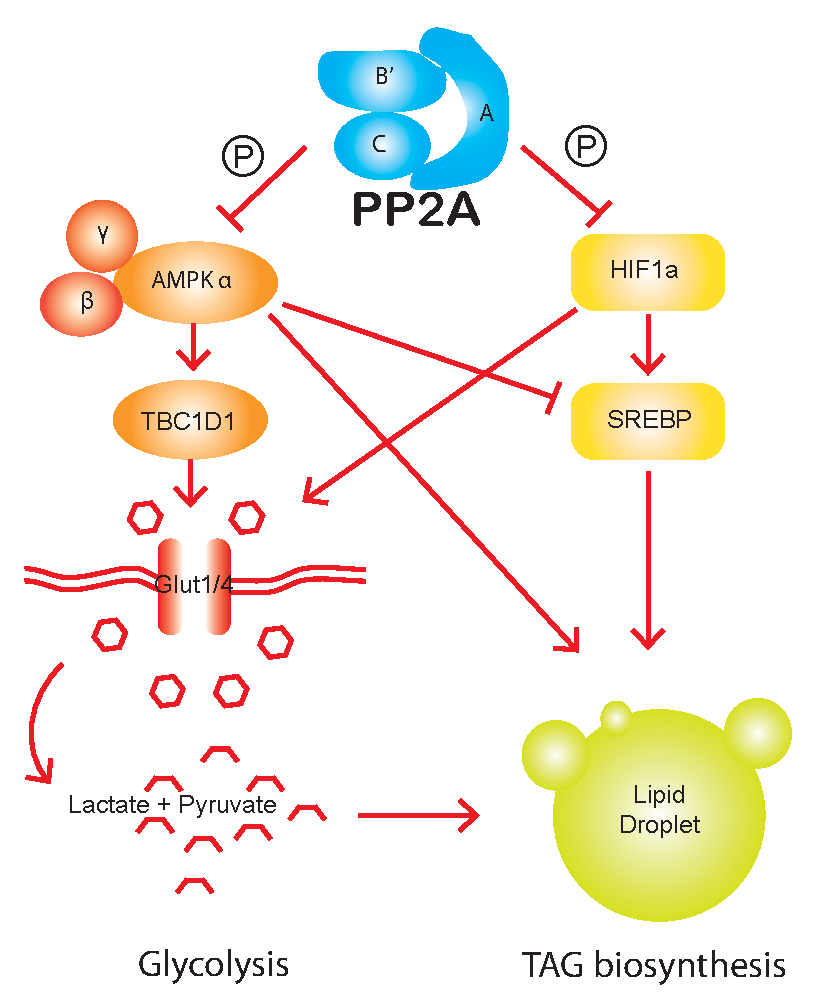
\includegraphics[width=0.8\textwidth]{figs/fig2-59 signaling model.png}
\caption[Cell-autonomous model for PPP2R5C in metabolic control]{\footnotesize Signaling model of PPP2R5C in glycolysis and lipogenesis in cell. PPP2R5C containing PP2A complex inhibits AMPK and HIF1\textalpha{} activity via de-phosphorylation. Although AMPK has been shown to be a negative regulator for SREBP-1 \cite{li_ampk_2011}, SREBP-1 could still be activated by the upstream HIF1\textalpha{} activation \cite{li_intermittent_2005} and potentially lower liver cholesterol in PPP2R5C knockdown at long term. Activated AMPK \cite{zhou_akt_2008,wu_ampk-dependent_2013,vichaiwong_contraction_2010} and HIF1\textalpha{} \cite{ochiai_disruption_2011,denko_hypoxia_2008} could both contribute to the increased glucose uptake and glycolysis in a cell-autonomous way. Even increased glycolysis itself could also contribute to \textit{de novo} lipogenesis \cite{hagiwara_hepatic_2012,foufelle_new_2002}. }
\label{fig:fig2.59}
\end{figure}

I have also evaluated the HIF1\textalpha{} phosphorylation  by Phos-tag\textsuperscript{\textregistered} gel since there was no commercially available phospho-specific antibody for HIF1\textalpha{}, and found its phosphorylation is increased upon PPP2R5C knockdown in Hepa 1-6 cell model. Concordantly, the HIF1\textalpha{} transcriptional activity is also up-regulated in mouse primary hepatocytes. These data indicate the functional consequence of HIF1\textalpha{} phosphorylation increase upon PPP2R5C KD could be the transcriptional activation of HIF1\textalpha{}. Further study would be needed to identify the phosphorylation site after PPP2R5C KD.  


The functional relevance of HIF1\textalpha{} is still less clear, given that the mice I was studying were housed under normoxia. Mice with liver-specific knockout of HIF1\textbeta{} developed diabetic phenotypes \cite{wang_ablation_2009}, however HIF1\textbeta{} binds also other partners besides HIF1\textalpha{}. The hepatocyte-specific knockout of HIF1\textalpha{} shows impaired glucose tolerance in Oral GTT testing \cite{ochiai_disruption_2011}, which is fit nicely with the improved glucose tolerance in PPP2R5C KD mice with potential HIF1\textalpha{} activation. In cell culture experiments with Hepa 1-6  cells or primary hepatocytes, also conducted under normoxia, HIF1\textalpha{} is indeed functionally relevant because I can detect the HIF1\textalpha{} protein by Western blot (\cref{fig:fig2.47,fig:fig2.51}) and see the induction of HIF1\textalpha{} target genes upon PPP2R5C knockdown (Figure~\ref{fig:fig2.53}). HIF1\textalpha{} is known to be frequently up-regulated and functionally relevant to cancers, therefore HIF1\textalpha{} is likely to be a relevant downstream PPP2R5C target in this pathophysiological context. Finally, the SREBP-1 activation was observed in PPP2R5C KD livers, which likely accounts for their increased \textit{de novo} lipogenesis. SREBP-1 can be activated downstream of HIF1\textalpha{} but additional mechanisms are likely to link PPP2R5C to SREBP-1 activation \cite{furuta_fatty_2008}. The lower cholesterol level in PPP2R5C KD liver could also explain the SREBP-1 activation. 

Besides these substrates identified in this project, other known interaction partners of PPP2R5C could also possibly contribute to the phenotypes after PPP2R5C KD, such as SERCA2a or SERCA3a identified in a proteomic search of PPP2R5C interaction proteins \cite{zhou_proteomic_2007}. In mammalian system, loss of the endogenous regulator of SERCA2a, sarcolipin, results in mice predisposed to diet-induced obesity \cite{bal_sarcolipin_2012}. Similarly, loss of \textit{Drosophilla} SERCA results fat accumulation in fat body of fly \cite{bi_seipin_2014}. The conserved function of SERCA family in lipid accumulation during evolution could be another plausible mechanism for increased lipogenesis phenotype upon PPP2R5C KD in hepatocytes. However, the phosphorylation of SERCA or ER calcium\textsuperscript{2+} level has to be examined in PPP2R5C KD cells in order to find the connection between PPP2R5C KD and SERCA-mediated signaling on lipogenesis.  



\section{PPP2R5C's metabolic control in cancer cells}

PPP2R5C has been linked to the cancer development. One mechanism in human appears to be the dephosphorylation of p53 on Thr55 \cite{li_specific_2007,shouse_serine_2008,nobumori_b56_2013}. However, this mechanism is not possible in the mouse due to the missing Thr55 in mouse p53. The results described here suggest an alternative mechanism for PPP2R5C's down-regulation in controlling cancer cell growth and proliferation by increasing the cancer cell glucose uptake, glycolytic rate, and lipid biosynthesis--all of which are metabolic hallmarks for cancer cells. This also fits with the tumor suppressor function of PPP2R5C, which is inhibiting the cell proliferation in cancer cells through reprogramming metabolism toward anabolic growth. Therefore, it will be interesting to study in the future whether these metabolic effects might be contributing towards the tumor suppressive properties of PPP2R5C in other tumor types besides hepatoma. 

As potential PPP2R5C substrate, HIF1\textalpha{} has been frequently stabilized and activated in solid tumor, and becomes the driving force for metabolic reprogramming toward "Warburg" effect by increasing glucose uptake and glycolysis \cite{denko_hypoxia_2008}. PPP2R5C's regulation on HIF1\textalpha{} provide a novel pathway to modulate HIF1\textalpha{} activity via phosphatase. Additionally, with recent advances in genome editing technology, it is now possible to specifically activate PPP2R5C expression with the help from CRISPR/Cas9 mediated genome-loci specific targeting and gene activation \cite{konermann_genome-scale_2014,qi_repurposing_2013}. Local activation of PPP2R5C in tumor cells would be a new perspective on drug development for cancer, turning PP2A a tumor suppressor as new druggable target for modulating HIF1\textalpha{} and other signaling pathways in cancer cells.

\section{PPP2R5C in human metabolic diseases}

From PPPR5C knockdown experiments, it has been clearly shown that PPP2R5C expression in the liver inhibits the glucose uptake and reduces the insulin sensitivity. Astoundingly, PPP2R5C expression level in human liver also correlates with insulin resistance. Type 2 diabetic patients have significantly elevated PPP2R5C liver expression levels compared to controls (Figure~\ref{fig:fig2.60}). In fact, even within the control population PPP2R5C expression correlates with reduced insulin sensitivity (Figure~\ref{fig:fig2.60}), raising the hypothesis for future studies that increased PPP2R5C expression might play a causative role in insulin resistance.

In type 1 or 2 diabetes, postprandial hyperglycemia and impaired hepatic glycogen storage are the two most prominent characteristics \cite{moore_regulation_2012}. Targeting postprandial glucose (PPG) level has also become a major interest in drug development for diabetes \cite{schrot_targeting_2004}. In fact, 2-hour GTT is still considered to be the gold standard for diagnosis of diabetes. And PPG has also been shown as frequently the earliest abnormality of type 2 diabetes, and an independent risk for cardiovascular diseases \cite{soonthornpun_postprandial_1999}. In this thesis project, liver-specific knockdown of PPP2R5C has been shown to induce profound metabolic changes, including increased insulin sensitivity without affect fasting blood glucose level, increased glucose uptake in GTT and consequently increased glycogen and triglyceride storage in the liver. PPP2R5C liver-specific knockdown has provided a new drug target for controlling PPG via multiple possible pathways. 

Either via liver-specific siRNA mediated knockdown or interrupting interactions between PPP2R5C and PP2A holoenzyme (A and C subunits), PPP2R5C's substrates can be specifically modulated in term of increasing their phosphorylation levels. Liver-specific siRNA delivery has been quite successful in recent studies \cite{wooddell_hepatocyte-targeted_2013,hattori_vivo_2014}. In the future, with more efficient and specific siRNA delivery system development, it is reasonable to test the clinical possibility of the liver-specific knockdown of PPP2R5C to improve postprandial hyperglycemia in diabetic patients. Currently, liver-specific knockdown of PPP2R5C in the mouse model of type 2 diabetes (\textit{db/db} mice) is ongoing. With the recent development in phosphatase-based drug development \cite{chatterjee_targeting_2013}, it is also plausible to develop activators or inhibitors for PP2A. Inhibitors, which could disrupt PPP2R5C's interaction with PP2A holoenzyme (A and C subunits) or specific substrates like AMPK or HIF1\textalpha{}, can be employed to target the liver and mimic the liver-specific knockdown effect on metabolic benefits for diabetes.





